\chapter{User Guide} \label{Guide}
% You must provide an adequate user guide for your software. The guide should provide easily understood instructions on how to use your software. A particularly useful approach is to treat the user guide as a walk-through of a typical session, or set of sessions, which collectively display all of the features of your package. Technical details of how the package works are rarely required. Keep the guide concise and simple. The extensive use of diagrams, illustrating the package in action, can often be particularly helpful. The user guide is sometimes included as a chapter in the main body of the report, but is often better included in an appendix to the main report.

\section{Opening Godot}

To run the projects in the .zip file, extract the projects into one folder. Then open Godot 4 (all projects in the source code listings folder are Godot 4 projects, \textbf{not} Godot 3 projects). When you start Godot for the first time, the project manager should be completely empty, without any projects, as described in Figure \ref{fig:godot1}. Projects have to be imported either one-by-one (by clicking ``Import" and going to the relevant project and opening it) or by clicking "Scan", then going to a folder of Godot projects and selecting it. The projects can then be opened in the project manager and edited as needed in Godot. Click ``Scan", then go to the folder where you extracted the projects, then click the ``Select Current Folder" button, as shown in Figure \ref{fig:godot2}, and all the projects should show up in the editor, as shown in Figure \ref{fig:godot3}. You can then double click on any one project (or click on it once and click the ``Edit" button) to open it in the Godot editor, an example of which is shown in Figure \ref{fig:godot4}. Alternatively, to run the project itself without opening the editor, using the currently saved values for exported script variables where appropriate, click on the project \textit{once} and click the ``Run" button.

\begin{figure}[H]
    \centering
    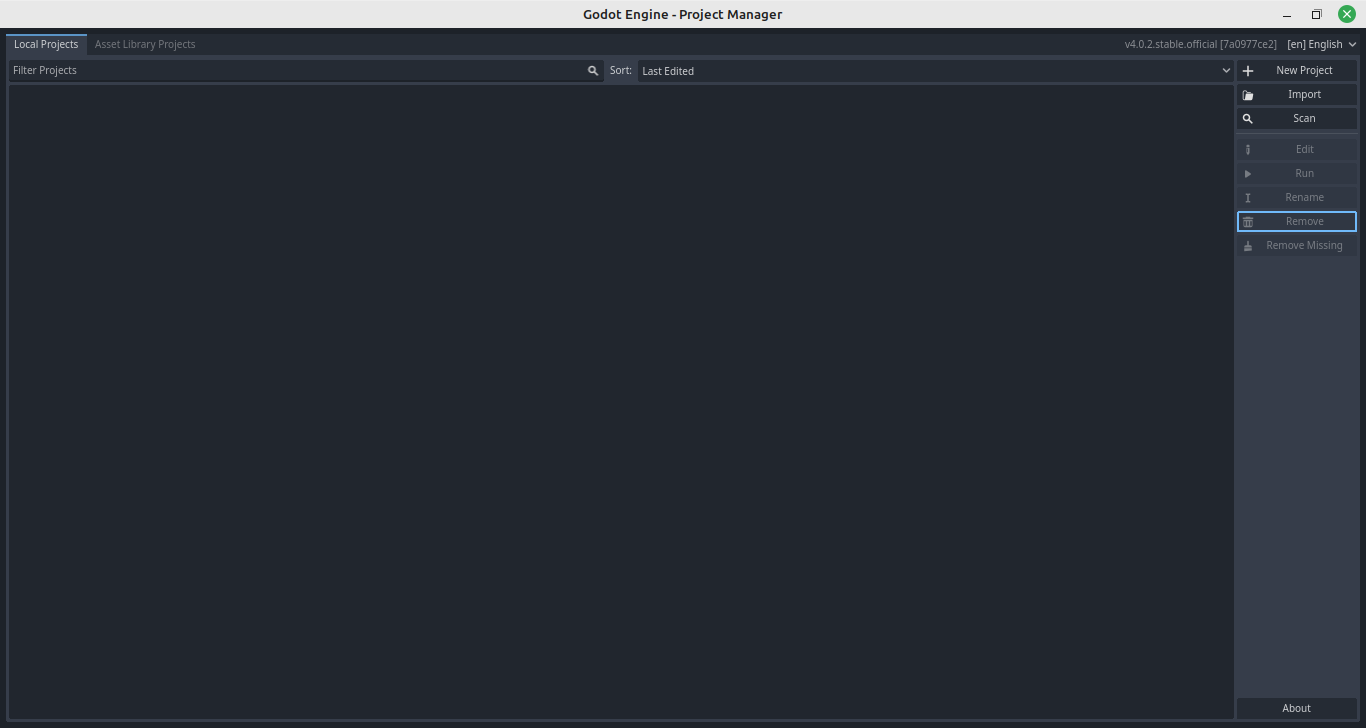
\includegraphics[width=\textwidth]{Images/open_godot.png}
    \caption{The Godot editor, when it is opened for the first time, does not show any projects in the editor (the Steam version bundles several example projects). Projects need to be imported either one-by-one or by scanning a folder of Godot projects.}
    \label{fig:godot1}
\end{figure}

\begin{figure}[H]
    \centering
    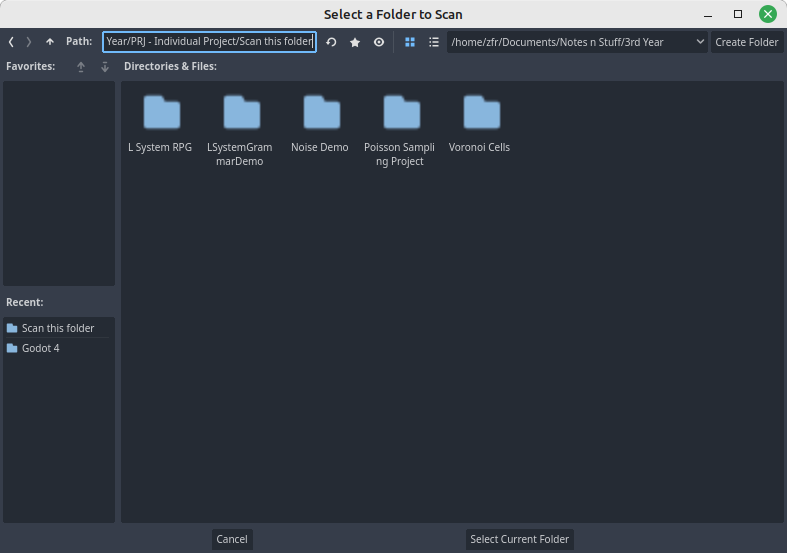
\includegraphics[width=\textwidth]{Images/scan-folder.png}
    \caption{You can click the "Scan" button in the project manager (in Figure \ref{fig:godot1}), then go to the relevant folder where your project are in Godot's built-in file explorer. Here, I have extracted my artefacts into a separate folder called ``Scan this folder" as an example.}
    \label{fig:godot2}
\end{figure}

\begin{figure}[H]
    \centering
    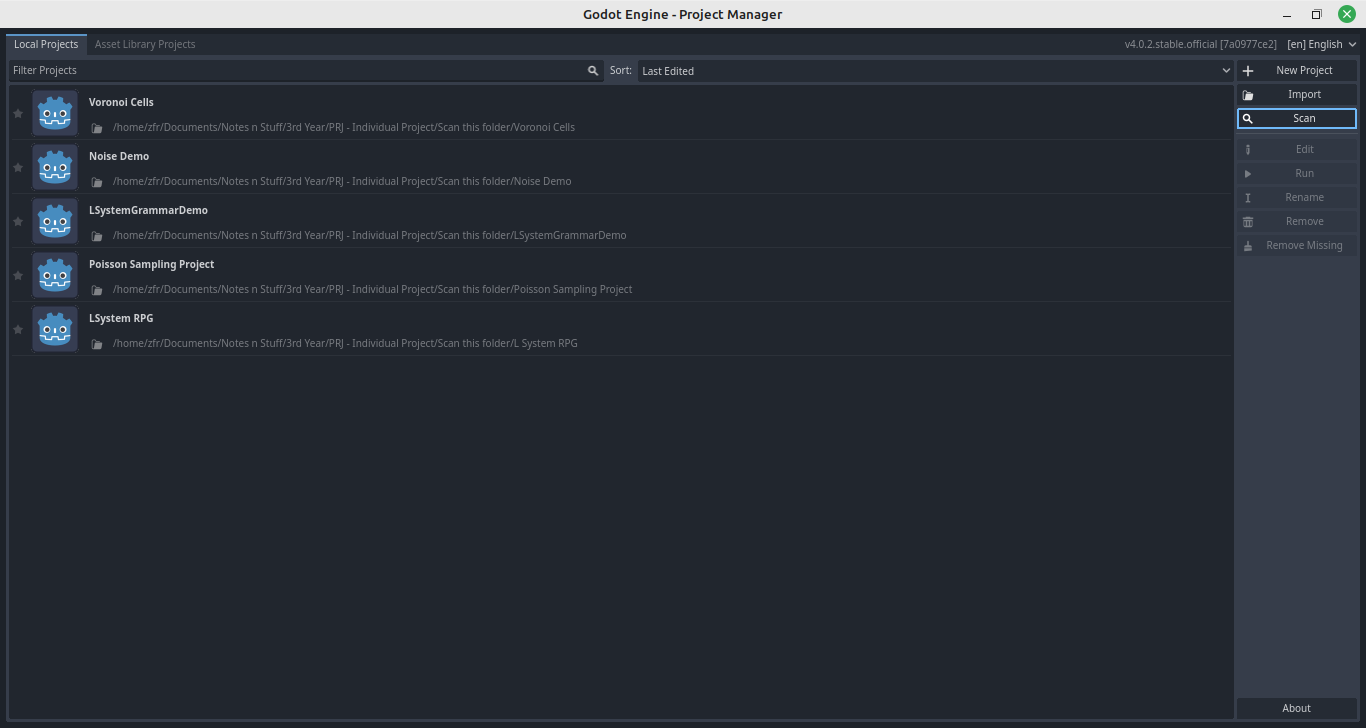
\includegraphics[width=\textwidth]{Images/projects-scanned.png}
    \caption{Once some Godot projects have been imported into the project manager, you should be able to easily view the list and double-click on any one of the projects to edit them, which will open the editor after closing the project manager. You could also click the ``Edit" button, or click ``Run" to run the game without having to open the editor itself.}
    \label{fig:godot3}
\end{figure}

\begin{figure}[H]
    \centering
    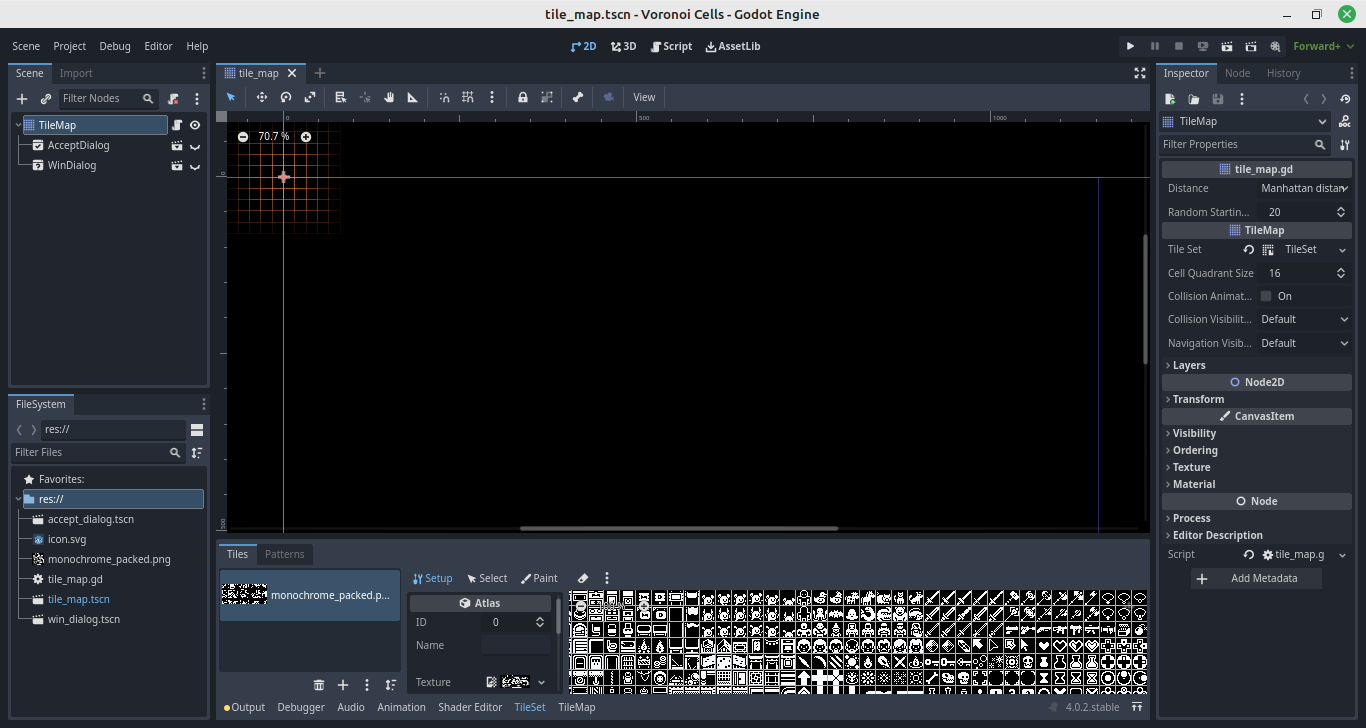
\includegraphics[width=\textwidth]{Images/godot-editor.png}
    \caption{The Godot editor open with the Voronoi cells project as an example. A visual description of the editor's contents is in chapter \ref{editor}.}
    \label{fig:godot4}
\end{figure}

\section{The Godot Editor} \label{editor}

As you open up the Godot editor, you will see the main scene view in the center, as shown in Figure \ref{fig:godot4}, using the Voronoi cells implementation as an example. The left-hand side shows the scene tree at the top, and the file system (from the root folder of the project) at the bottom. Meanwhile, the right hand side shows the currently selected node's export variables, \textit{including the custom export variables} defined in the node's script file, and two other tabs, ``Node" (which shows a list of signals for the scene that could be called in a script) and ``History" (which shows the sequence of recent actions performed on the scene during the current session). Above this is also a set of buttons which can be used for playing the project and/or the current scene. I go over how to run the current project in chapter \ref{runproject}.

\section{Custom Export Variables} 

When you click on some of the scenes in the projects, there may be some "exported" variables from scripts that are visible to you in the editor (examples include the "Distance" and "Random Starting Points" variables in the Voronoi Cells project). You can hover over the variable names in the editor and it will show a brief description of what the variable correlates to in the script. I go over the different export variables across all of my artefacts in this section.

\subsection{Lindenmayer System}

All of the custom export variables I defined for your use are in the child node ``LSystem" (it is saved into its own scene file, but it is cheifly a child node of the root node ``TileMap"). Open the ``TileMap" scene (if it is not already opened for you when you launch the Godot editor) and click on the ``LSystem" node in the scene tree to edit it.

\begin{enumerate}
    \item axiom
    \begin{itemize}
        \item \textbf{Type:} String
        \item \textbf{Documentation:} The starting string from which the grammar starts applying its rules. Here it may be self defined, or randomly defined when ``use\_random\_axiom" is true.
        \item \textbf{Default value:} ``OWB"
    \end{itemize}
    \item use\_random\_axiom
    \begin{itemize}
        \item \textbf{Type:} Boolean (bool) 
        \item \textbf{Documentation:} Uses a random axiom with the currently set grammar, computed upon runtime, with a length up to (but not strictly) the value of upper\_limit. For example, if upper\_limit is set to 15, the generated axiom can be 15 characters, or it can be just 5 characters.
        \item \textbf{Default value:} true
    \end{itemize}
    \item upper\_limit
    \begin{itemize}
        \item \textbf{Type:} Integer (int)
        \item \textbf{Documentation:} Defines how many characters a random axiom can have MAXIMUM. Only used when ``use\_random\_axiom" is true.
        \item \textbf{Default value:} 10
    \end{itemize}
    \item use\_custom\_ruleset
    \begin{itemize}
        \item \textbf{Type:} Boolean (bool)
        \item \textbf{Documentation:} Allows the use of a customly defined ruleset made through amending the rules array in the editor.
        \item \textbf{Default value:} false
    \end{itemize}
    \item ruleset
    \begin{itemize}
        \item \textbf{Type:} String enumeration of the following choices:
        \begin{enumerate}
            \item ``Default"
            \item ``More Buildings (IMPOSSIBLE)"
            \item ``More Trees"
            \item ``More Space"
        \end{enumerate}
        \item \textbf{Documentation:} Denotes a series of pre-defined rulesets for this L-System grammar, of alphabet O (blank space), W (trees and fauna) and B (buildings), that can be chosen and then used on runtime. Can choose between a default ruleset, a ruleset that produces more buildings, a ruleset that produces more trees and a ruleset that produces more empty space.
        \item \textbf{Default value:} ``Default"
    \end{itemize}
    \item rules
    \begin{itemize}
        \item \textbf{Type:} Array of dictionaries
        \item \textbf{Documentation:} The set of rules that the L-System grammar uses. Shows the ``default" ruleset in the Godot editor for the user to see. If ``use\_custom\_ruleset" is set to true, this array can be edited with a custom defined ruleset that will be used on runtime, so long as it adheres to the alphabet of O (blank space), W (trees and fauna) and B (buildings).
        \item \textbf{Additional information:} The ``\_get\_ruleset" function uses the String value in ``ruleset" to set the value for ``rules" on runtime, \textit{if} ``use\_custom\_ruleset" is false (which it \textit{is} by default).
        \item \textbf{Default value:} The ``Default" grammar, as shown in Figure \ref{fig:defaultgrammar}.
    \end{itemize}
\end{enumerate}

\begin{figure}[H]
    \centering
    \begin{lstlisting}
    [
    	{
    		"from": "O",
    		"to": "OWO"
    	},
    	{
    		"from": "W",
    		"to": "WB"
    	},
    	{
    		"from": "B",
    		"to": "BWO"
    	}
    ]
    \end{lstlisting}
    \caption{The ``Default" grammar used for the ``rules" export variable, stored in the constant ``DEFAULT" in l\_system.gd. See l\_system.gd for the other grammars represented as arrays of dictionaries.}
    \label{fig:defaultgrammar}
\end{figure}

\subsection{Perlin/Simplex Noise}

\begin{enumerate}
    \item noise\_type
    \begin{itemize}
        \item \textbf{Type:} String enumeration of the following choices:
        \begin{enumerate}
            \item ``Perlin"
            \item ``Simplex"
            \item ``Simplex Smooth"
            \item ``Value"
            \item ``Value Cubic"
        \end{enumerate}
        \item \textbf{Documentation:} Defines the type of noise generation algorithm to use. Equates to the ``noise\_type" property in FastNoiseLite.
        \item \textbf{Default value:} ``Value Cubic"
    \end{itemize}
    \item fractal\_type
    \begin{itemize}
        \item \textbf{Type:} Enumeration of the following choices:
        \begin{enumerate}
            \item ``Fractal None"
            \item ``Fractal FBM"
            \item ``Fractal Ridged"
            \item ``Fractal Ping Pong"
        \end{enumerate}
        \item \textbf{Documentation:} Defines the type of method used to combine octaves of a noise image into a fractal. Directly equates to the FractalType enumeration in FastNoiseLite.
        \item \textbf{Default value:} ``Fractal None" 
    \end{itemize}
    \item cellular\_distance\_type
    \begin{itemize}
        \item \textbf{Type:} Enumeration of the following choices:
        \begin{enumerate}
            \item ``Distance Euclidean"
            \item ``Distance Euclidean Squared"
            \item ``Distance Manhattan"
            \item ``Distance Hybrid"
        \end{enumerate}
        \item \textbf{Documentation:} Defines the function used to calculate the distance between the nearest/second-nearest point(s). Directly equates to the CellularDistanceFunction enumeration in FastNoiseLite.
        \item \textbf{Default value:} ``Distance Euclidean"
    \end{itemize}
    \item noise\_frequency
    \begin{itemize}
        \item \textbf{Type:} Floating point number (float) between 0.0 and 1.0 inclusive
        \item \textbf{Documentation:} Defines the frequency of the generated noise, the higher the frequency, the rougher and more granular the noise.
        \item \textbf{Additional information:} The default value for ``frequency" in the ``FastNoiseClass" is 0.01, resulting in very smooth and distinct noise. 
        \item \textbf{Default value:} 0.894
    \end{itemize}
    \item tree\_cap
    \begin{itemize}
        \item \textbf{Type:} Floating point number (float) between -1.0 and 1.0 inclusive
        \item \textbf{Documentation:} Defines the upper limit to set for painting a tree tile on a specific noise pixel. If the value returned by the ``get\_noise\_2d" method (in FastNoiseLite) is smaller than this, then it gets painted.
        \item \textbf{Default value:} -0.048
    \end{itemize}
    \item building\_cap
    \begin{itemize}
        \item \textbf{Type:} Floating point number (float) between -1.0 and 1.0 inclusive
        \item \textbf{Documentation:} Defines the upper limit to set for painting a building tile on a specific noise pixel. If the value returned by the ``get\_noise\_2d" method (in FastNoiseLite) is smaller than this, then it gets painted. If the value of ``building\_cap" is smaller than ``tree\_cap," then decide whether or not to paint a building cell there with ``building\_overtakes\_tree."
        \item \textbf{Default value:} -0.252
    \end{itemize}
    \item building\_overtakes\_tree
    \begin{itemize}
        \item \textbf{Type:} Floating point number (float) between 0.0 and 0.5 inclusive
        \item \textbf{Documentation:} Only used when ``building\_cap" is smaller than ``tree\_cap." Determines the probability that a building tile would be painted in a cell where a tree tile was, or could be, also painted. Whether or not the cell actually is painted over is decided on computation time.
        \item \textbf{Default value:} 0.12
    \end{itemize}
\end{enumerate}

\subsection{Poisson Disk Sampling}

\begin{enumerate}
    \item paint\_building\_probability
    \begin{itemize}
        \item \textbf{Type:} Floating point number (float) between 0.0 and 1.0 inclusive
        \item \textbf{Documentation:} The probability that a building gets painted at a cell in lieu of a tree. The higher this probability, the more likely a building tile gets painted instead of a tree tile. 
        \item \textbf{Default value:} 0.125
    \end{itemize}
    \item point\_radius
    \begin{itemize}
        \item \textbf{Type:} Floating point number (float) between 0.5 and 2.5 inclusive
        \item \textbf{Documentation:} The radius value used to measure distances between points for the algorithm. The longer the radius, the further apart points are during the algorithm's processing, and the further apart painted cells are in the game.
        \item \textbf{Default value:} 1.0
    \end{itemize}
    \item region\_size
    \begin{itemize}
        \item \textbf{Type:} Vector2
        \item \textbf{Documentation:} The size of the region in which the algorithm is performed. Set to the "default" tile map size (72, 40) in the script, shown as (0, 0) in the Godot editor. Can be changed to use a smaller region for the algorithm itself, of course resulting in less cells covered within the boundaries set for this game, though the algorithm will perform faster due to less cells being checked.
        \item \textbf{Default value:} 
        \begin{itemize}
            \item \textbf{x}: The value in ``x\_tile\_range" (72)
            \item \textbf{y}: The value in ``y\_tile\_range" (40)
        \end{itemize}
    \end{itemize}
    \item rejection\_samples
    \begin{itemize}
        \item \textbf{Type:} Integer (int) between 1 andc 50 inclusive
        \item \textbf{Documentation:} The maximum number of times a cell is checked before it is ignored. A cell can be accepted and painted on before this maximum number is reached. The higher this value, the more times a cell is checked, therefore the higher the algorithm's processing time.
        \item \textbf{Default value:} 8
    \end{itemize}
\end{enumerate}

\subsection{Voronoï Cells}

\begin{enumerate}
    \item distance
    \begin{itemize}
        \item \textbf{Type:} String enumeration of the following choices:
        \begin{enumerate}
            \item ``Euclidean distance"
            \item ``Manhattan distance"
        \end{enumerate}
        \item \textbf{Documentation:} Determines whether or not the Euclidean or Manhattan distance formula is used for calculation of the deltas between points within Voronoi cells.
        \item \textbf{Default value:} ``Manhattan distance"
    \end{itemize}
    \item random\_starting\_points
    \begin{itemize}
        \item \textbf{Type:} Integer (int) between 15 and 40 inclusive
        \item \textbf{Documentation:} Determines the number of points randomly picked from at the start. Therefore, it also determines the number of cells in our Voronoi tesselation.
        \item \textbf{Default value:} 20
    \end{itemize}
\end{enumerate}

\subsection{The Basic L-System Demo Used to Create the Screenshots in Chapter \ref{alglsys}}

There is only one export variable for this: ``choices", which allows you to choose which one of the three provided rulesets to use. ``choices" is the default ruleset, and either ``deterministic" or ``basic" can be chosen. It is in the ``DemoNode" scene, the only scene of this Godot project. Quoting the documentation comment, this export variable ``Allows you to decide which ruleset to use. See the script file for the sources of said rulesets." The ruleset is assigned with the ``set\_values" function.

\newpage

\section{Running the Godot Projects} \label{runproject}

To \textit{run} the current project in the Godot editor, go to the bar above the Inspector, Node and History tabs on the right-hand side. You will find a \faPlay{} button which will play the main scene of the project (in my artefacts, the main scenes have already been set; if it were not already set, you would have been asked to set one). If closing the window to stop the project does not work, hit the \faStop{} button to end it. 

As described in section \ref{commonalities}, only the close button of both the popup dialogs in the game seems to work properly for the moment, but this does not adversely affect the game functioning properly, nor does it adversely affect this project, so this is trivial.
